\documentclass{article}
\usepackage[margin=1in]{geometry}
\usepackage{../common}
\usepackage{../pagesetup}
% **** IF YOU WANT TO DEFINE ADDITIONAL MACROS FOR YOURSELF, PUT THEM HERE:

\begin{document}

\lecture{13}{October 18}{Sasha Rush}{Peter Chang, Ruiqi Chen, Joonhee Choi, Joshua Meier, Raphael Rouvinov, Hyungmok Son}{Information Theory}

\subsection{Announcements}
The Midterm is next Monday. The list of topics is on the website. It's open note but not open computer. You can bring your textbook. They'll try to bring copies of the textbook for people who don't have it so they don't have to print out copies. 

\subsection{Introduction}
Interestingly, almost all of information theory is laid out in a single paper, written by Claude Shannon in 1948. We often quote Alan Turing as the 'father' of CS, but for the area we are discussing, that 'father' is Shannon. (Aside: \href{https://www.youtube.com/watch?v=cZ34RDn34Ws}{Video of device Shannon built called the Ultimate Machine})

\smallskip
Today, we'll cover the core aspects of information theory and discuss how we'll use it in this class.

\smallskip
Earlier in this class, we've focused on exact methods for inference: MLE, MAP, etc. The one exception was neural networks, which are not convex.

\smallskip
Exact inference is only tractable in a small subset of models. Given most models are intractable, what do we do? We use approximate inference. Here, there are two main types of approximation:  optimization-based (which includes coordinate ascent, SGD, and Linear Programming methods) and sample-based. You can use them together, but they have different histories, so we'll discuss them separately. 

\smallskip
Information theory brings together many of the expectation-maximization methods we've seen earlier into a unified language. In particular, information theory lets us study relative entropy.

\subsection{Information theory (Murphy 2.8)}
\begin{center}
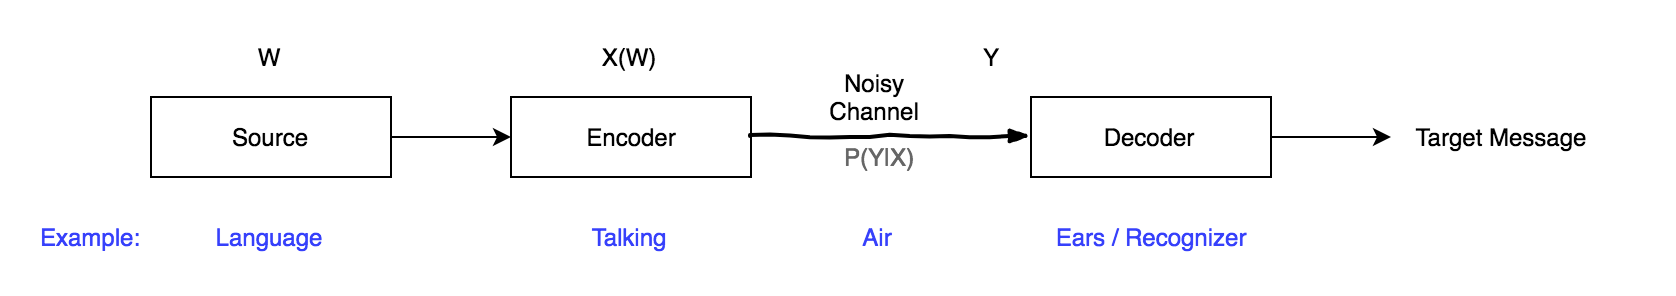
\includegraphics[width=\textwidth]{IT-diagram.png}
\end{center}
The \textit{Information Source} spits out bits (call this W), which is passed into the \textit{encoder} (giving X(W)). The encoded bits pass through a \textit{noisy channel} giving Y, which is passed into a \textit{decoder} that gives us our target message.

\smallskip
We don't know how the noisy channel will act in a deterministic way. But we have a probability distribution $p(Y|X)$ describing its behavior. The target message also has a distribution $p(x|y) \ \alpha \ p(x) p(y|x)$. Where $p(x)$ represents the source model, and $p(y|x)$ represents the channel model. We have a simple graphical model here:

\begin{center}
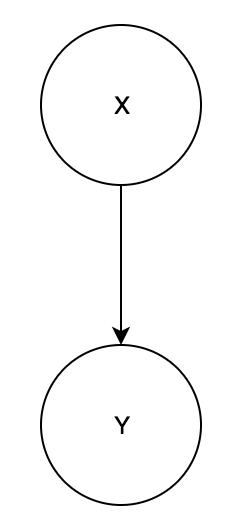
\includegraphics[width=0.75in]{g-model.png}
\end{center}


\smallskip
Several fields of research are contained in the first diagram. One area of information theory is called channel coding (Noisy Channel in diagram). It studies how to best encode the data so it is most robust to the noisy channel. A second area is called source coding - data compression (Source in diagram). It discusses how we can exploit the way information is naturally represented in the world. For example, compression falls here. (Aside: \href{http://prize.hutter1.net/}{Hutter prize}).

\smallskip
\textbf{Example}: people in speech recognition use this as an analogy for what they are trying to do. The model of what a person wants to say is $W$. The encoding path is the sound the person makes $X(w)$. The decoder is what we (or the microphone) hear. And the goal, of course, is to uncover the target message.

\smallskip
We can write this analogy:
\begin{enumerate}
\item Source: Language
\item Encoder: Talking
\item Noisy Channel: Air
\item Decoder: ears/recognizer
\end{enumerate}

\smallskip
Then, $p(X)$ represents the source model. If you know a person well, you can anticipate what is going on in their head, and you know what they are going to say This makes your $p(X|Y)$ stronger. We multiply this quantity by $p(Y|X)$ which represents the noisiness of the channel.

\subsection{Definitions}

\textbf{Entropy:}

$$H(X) \overset{\Delta}{=}  - \sum_{k=1}^K p(x=k) \log_2 p(x = k) = -E_k[\log_2 p(x=k)]$$
For a given random variable $X$, entropy measures the "uncertainty" in the distribution. Entropy maxes out when we have full uncertainty in the distribution. 

\begin{figure}[h!]
\centering
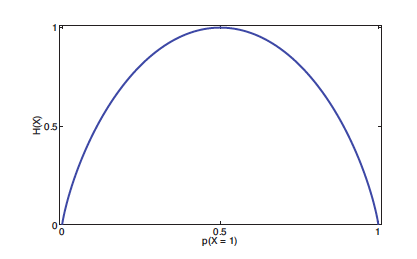
\includegraphics[scale=0.45]{parabola.png}
\label{fig:univerise}
\end{figure}

\pagebreak
\smallskip
This comes back to the idea of source coding. If there is full certainty in what can and is sent, then it does not matter what the encoder/decoder does. The answer is trivial. In contrast, if there is full uncertainty, we have to work much harder.

\smallskip
The unit of measure of this is called "bits"($\log_2$) or "shannons" or "nats" ($\log_e$). The average number of bits needed to represent a message is less than $$H(x) + 1$$ We won't prove this, but this is the fundamental link between information and coding.

\smallskip
\smallskip
\textbf{Shannon Game}
In his paper, Shannon proposes the "Shannon Game," which tries to quantify human source coding: given a sequence of text, give a probability distribution over the next letter/word.

\smallskip
THE ROOM WAS NOT VERY LIGHT A SMALL OBLONG READING LAMP ON THE DESK SHED GLOW ON POLISHED \_\_\_.

\smallskip
\smallskip
In English, it takes roughly 80 guesses to get the right answer. We write that the perplexity or "how confusing the next prediction is" is
$$2^{H(x)}$$

Minimizing perplexity is where the 'power'/advances of RNNs comes from.

\smallskip
\textbf{Cross Entropy:}

\begin{enumerate}
\item $p$ - is a true underlying distribution
\item $q$ - another distribution that approximates $p$
\end{enumerate}

$$H(p, q) = - \sum_k p(x=k) \log q(x=k) = E_p[\log q(x=k)]$$

Cross entropy tells us expected number of bits to encode true distribution $p$ with $q$.

\smallskip
We can sample from $p$ to approximate
$$\tilde{x_1}, \ldots, \tilde{x_N} \sim p(x)$$
Then, we compute the minimization of the cross entropy.
$$min_q - \frac{1}{n} \sum_{n}^N \log q(\tilde{x_n})$$

\smallskip
But this is just the negative log likelihood for categoricals. Last class, we talked about RNNs. We learn $q$ and compare to $p$. If we can make it more and more like $p$, this gives us the ability to do compression and source modeling better.


\smallskip 
\smallskip
\textbf{Relative entropy (KL-Divergence):}

$$KL(p || q) \overset{\Delta}{=} E_p \log \frac{p_(x=k)}{p(q=k)} = \sum_k p_k \log \frac{p_k}{q_k} = \sum_k p_k \log p_k - \sum_k p_k \log q_k = -H(p) + H(p,q)$$

So the relative entropy is the negative entropy of $p$ by itself plus the relative entropy of $p$ and $q$. It's a way of comparing two distributions, but is not a metric - $KL(p || q) \neq KL(q || p)$

\smallskip
\smallskip
\textit{Theorem}. $KL(p||q) \geq 0$

\textit{Proof}. We have that
$$-KL(p||q) = E_p [\log \frac{q_k}{p_k}] \leq \log E_p[ \frac{q_k}{p_k} ] = \log \sum_k q_k(x) = \log 1 = 0$$
This is only $KL(p||q) = 0$ when $p = q$. 

\smallskip
\smallskip
\textit{Jensen's Inequality.}
$$f(E[x]) \leq E[f(x)]$$
if $f$ is convex. Mostly using when $f = \log$. 

\smallskip
\smallskip
\textbf{Information Geometry (Working with asymmetrical divergence).}

We have some $p$ and want $q \in Q$ (set of distributions). There are two options: 

\smallskip
\textit{1. Forward (moment projection):}

$$argmin_{q \in Q} KL(p||q) = -H(p) + H(p,q)$$
Note that $H(p)$ falls out when minimizing $q$. So instead, we minimize at $H(p,q)$, which is the negative log likelihood. So essentially, we are matching the moments. This equals $$-E_p \log q_k$$

\smallskip
Issues arise when $q_k \rightarrow 0$ and $p_k >0$. Forward projection will try to avoid zeros.

\smallskip
\smallskip
\textit{2. Reverse (information projection):}

$$argmin_{q \in Q} KL(q||p) = -H(q) + H(q, p) = -H(q) + E_q \log p_k$$
This method "matches the modes".

\smallskip
Issues arises when $p_k = 0$ and $q_k = 0$. Reverse projection will over predict zeros.

\smallskip
These two approaches fall under a field called Information Geometry.
The forward approach is called moment projection. The backward approach is called information projection. "Essentially, these are both methods for computing closeness among different distributions."

\smallskip
 \textit{Jensen-Shannon divergence} -- combine the above: add half of the Forward projection value to half of the reverse projection value. This approach is popular right now. 
 
\smallskip
This work is highly related to Generative Adversarial Networks (GANs). This metric is important in producing non-blurry images. Combining two images looks bad, using a method with mode finding yields a better image.

\subsection{Demo}

\smallskip
We did an example iPython notebook (KL.ipynb) in class.

\smallskip
Next class, we will use the reverse projection to get Q. This is called "variational inference".

\end{document}
